\documentclass[]{article}
\usepackage{lmodern}
\usepackage{amssymb,amsmath}
\usepackage{ifxetex,ifluatex}
\usepackage{fixltx2e} % provides \textsubscript
\ifnum 0\ifxetex 1\fi\ifluatex 1\fi=0 % if pdftex
  \usepackage[T1]{fontenc}
  \usepackage[utf8]{inputenc}
\else % if luatex or xelatex
  \ifxetex
    \usepackage{mathspec}
  \else
    \usepackage{fontspec}
  \fi
  \defaultfontfeatures{Ligatures=TeX,Scale=MatchLowercase}
\fi
% use upquote if available, for straight quotes in verbatim environments
\IfFileExists{upquote.sty}{\usepackage{upquote}}{}
% use microtype if available
\IfFileExists{microtype.sty}{%
\usepackage{microtype}
\UseMicrotypeSet[protrusion]{basicmath} % disable protrusion for tt fonts
}{}
\usepackage[margin=1in]{geometry}
\usepackage{hyperref}
\hypersetup{unicode=true,
            pdftitle={Markdown},
            pdfborder={0 0 0},
            breaklinks=true}
\urlstyle{same}  % don't use monospace font for urls
\usepackage{color}
\usepackage{fancyvrb}
\newcommand{\VerbBar}{|}
\newcommand{\VERB}{\Verb[commandchars=\\\{\}]}
\DefineVerbatimEnvironment{Highlighting}{Verbatim}{commandchars=\\\{\}}
% Add ',fontsize=\small' for more characters per line
\usepackage{framed}
\definecolor{shadecolor}{RGB}{248,248,248}
\newenvironment{Shaded}{\begin{snugshade}}{\end{snugshade}}
\newcommand{\KeywordTok}[1]{\textcolor[rgb]{0.13,0.29,0.53}{\textbf{#1}}}
\newcommand{\DataTypeTok}[1]{\textcolor[rgb]{0.13,0.29,0.53}{#1}}
\newcommand{\DecValTok}[1]{\textcolor[rgb]{0.00,0.00,0.81}{#1}}
\newcommand{\BaseNTok}[1]{\textcolor[rgb]{0.00,0.00,0.81}{#1}}
\newcommand{\FloatTok}[1]{\textcolor[rgb]{0.00,0.00,0.81}{#1}}
\newcommand{\ConstantTok}[1]{\textcolor[rgb]{0.00,0.00,0.00}{#1}}
\newcommand{\CharTok}[1]{\textcolor[rgb]{0.31,0.60,0.02}{#1}}
\newcommand{\SpecialCharTok}[1]{\textcolor[rgb]{0.00,0.00,0.00}{#1}}
\newcommand{\StringTok}[1]{\textcolor[rgb]{0.31,0.60,0.02}{#1}}
\newcommand{\VerbatimStringTok}[1]{\textcolor[rgb]{0.31,0.60,0.02}{#1}}
\newcommand{\SpecialStringTok}[1]{\textcolor[rgb]{0.31,0.60,0.02}{#1}}
\newcommand{\ImportTok}[1]{#1}
\newcommand{\CommentTok}[1]{\textcolor[rgb]{0.56,0.35,0.01}{\textit{#1}}}
\newcommand{\DocumentationTok}[1]{\textcolor[rgb]{0.56,0.35,0.01}{\textbf{\textit{#1}}}}
\newcommand{\AnnotationTok}[1]{\textcolor[rgb]{0.56,0.35,0.01}{\textbf{\textit{#1}}}}
\newcommand{\CommentVarTok}[1]{\textcolor[rgb]{0.56,0.35,0.01}{\textbf{\textit{#1}}}}
\newcommand{\OtherTok}[1]{\textcolor[rgb]{0.56,0.35,0.01}{#1}}
\newcommand{\FunctionTok}[1]{\textcolor[rgb]{0.00,0.00,0.00}{#1}}
\newcommand{\VariableTok}[1]{\textcolor[rgb]{0.00,0.00,0.00}{#1}}
\newcommand{\ControlFlowTok}[1]{\textcolor[rgb]{0.13,0.29,0.53}{\textbf{#1}}}
\newcommand{\OperatorTok}[1]{\textcolor[rgb]{0.81,0.36,0.00}{\textbf{#1}}}
\newcommand{\BuiltInTok}[1]{#1}
\newcommand{\ExtensionTok}[1]{#1}
\newcommand{\PreprocessorTok}[1]{\textcolor[rgb]{0.56,0.35,0.01}{\textit{#1}}}
\newcommand{\AttributeTok}[1]{\textcolor[rgb]{0.77,0.63,0.00}{#1}}
\newcommand{\RegionMarkerTok}[1]{#1}
\newcommand{\InformationTok}[1]{\textcolor[rgb]{0.56,0.35,0.01}{\textbf{\textit{#1}}}}
\newcommand{\WarningTok}[1]{\textcolor[rgb]{0.56,0.35,0.01}{\textbf{\textit{#1}}}}
\newcommand{\AlertTok}[1]{\textcolor[rgb]{0.94,0.16,0.16}{#1}}
\newcommand{\ErrorTok}[1]{\textcolor[rgb]{0.64,0.00,0.00}{\textbf{#1}}}
\newcommand{\NormalTok}[1]{#1}
\usepackage{graphicx,grffile}
\makeatletter
\def\maxwidth{\ifdim\Gin@nat@width>\linewidth\linewidth\else\Gin@nat@width\fi}
\def\maxheight{\ifdim\Gin@nat@height>\textheight\textheight\else\Gin@nat@height\fi}
\makeatother
% Scale images if necessary, so that they will not overflow the page
% margins by default, and it is still possible to overwrite the defaults
% using explicit options in \includegraphics[width, height, ...]{}
\setkeys{Gin}{width=\maxwidth,height=\maxheight,keepaspectratio}
\IfFileExists{parskip.sty}{%
\usepackage{parskip}
}{% else
\setlength{\parindent}{0pt}
\setlength{\parskip}{6pt plus 2pt minus 1pt}
}
\setlength{\emergencystretch}{3em}  % prevent overfull lines
\providecommand{\tightlist}{%
  \setlength{\itemsep}{0pt}\setlength{\parskip}{0pt}}
\setcounter{secnumdepth}{0}
% Redefines (sub)paragraphs to behave more like sections
\ifx\paragraph\undefined\else
\let\oldparagraph\paragraph
\renewcommand{\paragraph}[1]{\oldparagraph{#1}\mbox{}}
\fi
\ifx\subparagraph\undefined\else
\let\oldsubparagraph\subparagraph
\renewcommand{\subparagraph}[1]{\oldsubparagraph{#1}\mbox{}}
\fi

%%% Use protect on footnotes to avoid problems with footnotes in titles
\let\rmarkdownfootnote\footnote%
\def\footnote{\protect\rmarkdownfootnote}

%%% Change title format to be more compact
\usepackage{titling}

% Create subtitle command for use in maketitle
\newcommand{\subtitle}[1]{
  \posttitle{
    \begin{center}\large#1\end{center}
    }
}

\setlength{\droptitle}{-2em}

  \title{Markdown}
    \pretitle{\vspace{\droptitle}\centering\huge}
  \posttitle{\par}
    \author{}
    \preauthor{}\postauthor{}
    \date{}
    \predate{}\postdate{}
  

\begin{document}
\maketitle

Markdown is a simple formatting syntax for authoring HTML, PDF, and MS
Word documents. For more details on using R Markdown see
\url{http://rmarkdown.rstudio.com}. This document was produced using R
Markdown.

When you click the \textbf{Knit} button in RStudio a document will be
generated that includes both content as well as the output of any
embedded R code chunks within the document. You can embed an R code
chunk like this:

\begin{Shaded}
\begin{Highlighting}[]
\KeywordTok{summary}\NormalTok{(cars)}
\end{Highlighting}
\end{Shaded}

\begin{verbatim}
##      speed           dist       
##  Min.   : 4.0   Min.   :  2.00  
##  1st Qu.:12.0   1st Qu.: 26.00  
##  Median :15.0   Median : 36.00  
##  Mean   :15.4   Mean   : 42.98  
##  3rd Qu.:19.0   3rd Qu.: 56.00  
##  Max.   :25.0   Max.   :120.00
\end{verbatim}

You can also embed plots, for example:

\includegraphics{RMarkdown__1__files/figure-latex/unnamed-chunk-2-1.pdf}

Note that the \texttt{echo\ =\ FALSE} parameter was added to the code
chunk to prevent printing of the R code that generated the plot.

In answering assignment questions, incorporate mathematics,
\texttt{R\ code}, and plots as appropriate.

For example, using \texttt{RMarkdown} from \texttt{RStudio}, you might
have something inline showing like this \texttt{qt(0.9,\ 64)} and
evaluated like this 1.2949198.

You will also want to include whole chunks of code and output like this:

\begin{Shaded}
\begin{Highlighting}[]
\NormalTok{n <-}\StringTok{ }\DecValTok{40}
\NormalTok{x <-}\StringTok{ }\KeywordTok{runif}\NormalTok{(n, }\DataTypeTok{min=}\OperatorTok{-}\DecValTok{2}\NormalTok{, }\DataTypeTok{max=}\DecValTok{2}\NormalTok{)}
\NormalTok{y <-}\StringTok{ }\NormalTok{x}\OperatorTok{^}\DecValTok{2} \OperatorTok{+}\StringTok{ }\KeywordTok{rnorm}\NormalTok{(n, }\DataTypeTok{sd=}\FloatTok{0.2}\NormalTok{)}
\KeywordTok{plot}\NormalTok{(x,y, }\DataTypeTok{pch=}\DecValTok{19}\NormalTok{, }\DataTypeTok{col=} \KeywordTok{adjustcolor}\NormalTok{(}\StringTok{"firebrick"}\NormalTok{, }\DataTypeTok{alpha.f=}\FloatTok{0.7}\NormalTok{))}
\end{Highlighting}
\end{Shaded}

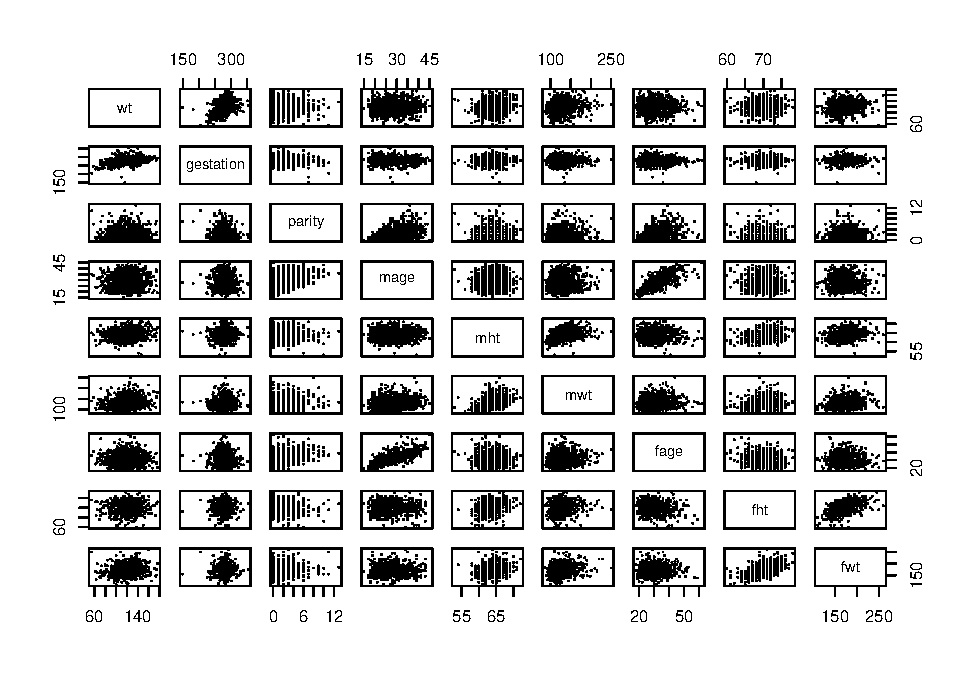
\includegraphics{RMarkdown__1__files/figure-latex/unnamed-chunk-3-1.pdf}

And then have your discussion appear around the code and the plot it
produced.

Alternatively you might want to just show the code, without evaluating
it.

\begin{Shaded}
\begin{Highlighting}[]
\NormalTok{n <-}\StringTok{ }\DecValTok{40}
\NormalTok{x <-}\StringTok{ }\KeywordTok{runif}\NormalTok{(n, }\DataTypeTok{min=}\OperatorTok{-}\DecValTok{2}\NormalTok{, }\DataTypeTok{max=}\DecValTok{2}\NormalTok{)}
\NormalTok{y <-}\StringTok{ }\NormalTok{x}\OperatorTok{^}\DecValTok{2} \OperatorTok{+}\StringTok{ }\KeywordTok{rnorm}\NormalTok{(n, }\DataTypeTok{sd=}\FloatTok{0.2}\NormalTok{)}
\KeywordTok{plot}\NormalTok{(x,y, }\DataTypeTok{pch=}\DecValTok{19}\NormalTok{, }\DataTypeTok{col=} \KeywordTok{adjustcolor}\NormalTok{(}\StringTok{"firebrick"}\NormalTok{, }\DataTypeTok{alpha.f=}\FloatTok{0.7}\NormalTok{))}
\end{Highlighting}
\end{Shaded}

Or evaluate it but not show it

\includegraphics{RMarkdown__1__files/figure-latex/unnamed-chunk-5-1.pdf}

You might also want to be a bit particular about any figure you produce:

\begin{Shaded}
\begin{Highlighting}[]
\NormalTok{n <-}\StringTok{ }\DecValTok{40}
\NormalTok{x <-}\StringTok{ }\KeywordTok{runif}\NormalTok{(n, }\DataTypeTok{min=}\OperatorTok{-}\DecValTok{2}\NormalTok{, }\DataTypeTok{max=}\DecValTok{2}\NormalTok{)}
\NormalTok{y <-}\StringTok{ }\NormalTok{x}\OperatorTok{^}\DecValTok{2} \OperatorTok{+}\StringTok{ }\KeywordTok{rnorm}\NormalTok{(n, }\DataTypeTok{sd=}\FloatTok{0.2}\NormalTok{)}
\KeywordTok{plot}\NormalTok{(x,y, }\DataTypeTok{pch=}\DecValTok{19}\NormalTok{, }\DataTypeTok{col=} \KeywordTok{adjustcolor}\NormalTok{(}\StringTok{"firebrick"}\NormalTok{, }\DataTypeTok{alpha.f=}\FloatTok{0.7}\NormalTok{))}
\end{Highlighting}
\end{Shaded}

\begin{center}\includegraphics{RMarkdown__1__files/figure-latex/unnamed-chunk-6-1} \end{center}

\textbf{Some Math}

It might, or might not, include some mathematics inline like this
\(\mu({\bf x})\) or this \(\frac{\pi}{2}\), using \$ around the texts
or, using \$\$ as a separate block like this \[
Y_{new} - \widetilde{\mu}({\bf x}_{new}) \sim N\left(0 ~,~ \sigma^2 \left( 1 + {\bf x}_{new}^T\left( {\bf X}^T{\bf X} \right)^{-1}
                      {\bf x}_{new} \right) \right).
\] or even a multi-equation block like: \[
\begin{array}{rcl}
\alpha & = & Pr\left(-a ~\le~ 
\frac{ Y_{new} - \widetilde{\mu}({\bf x}_{new}) 
              }
     {\widetilde{\sigma} \sqrt{ 1 ~+~
      {\bf x}^T_{new}
             \left( {\bf X}^T{\bf X} \right)^{-1}
             {\bf x}_{new}
             }
     }
     \le ~a~ \right) \\
&& \\
&=& Pr \left(~ {\bf I}_{new}({\bf x}_{new})
            \ni Y_{new} 
        ~\right)
\end{array}
\]

You could also have used a different indicator for equations namely
``\textbackslash{}{[}" and ``\textbackslash{}{]}''.

Here are a couple of other examples: \[
x_i = 
\left\{  \begin{array}{lcl}
          1  & ~~~~~~ & \text{if } i \text{  is odd} \\
          &&\\
          0 & & \text{otherwise.}
          \end{array}
\right.
\] and \[
\mathbf{X} = 
\left[ \begin{array}{cc}
a & b \\
&\\
c&d \\
&\\
3 & e 
\end{array}
\right]
\] Make your answers complete, as if they were a report on your
findings.

To include images:

\begin{figure}
\centering
\includegraphics{figure.png}
\caption{Moving a plane through 3d}
\end{figure}

To include a link\\
\color{blue} \href{http://www.chrisjordan.com/gallery/rtn2/\#tuna}{Chris
Jordan runs the numbers} \color{black}

For miscellaneous other info, see \color{blue}
\href{http://rmarkdown.rstudio.com/authoring_basics.html}{RStudio's
RMarkdown Basics} \color{black} or their \color{blue}
\href{https://www.rstudio.com/wp-content/uploads/2015/02/rmarkdown-cheatsheet.pdf}{cheatsheet}
\color{black} and \color{blue}
\href{https://www.rstudio.com/wp-content/uploads/2015/03/rmarkdown-reference.pdf}{reference
guide}\color{black}.


\end{document}
